\documentclass{article}
\usepackage{cmap}
\usepackage[utf8]{inputenc}
\usepackage[english,ukrainian]{babel}
\usepackage{graphicx}
\usepackage{geometry}
\usepackage{listings}
\usepackage{amsmath}
\usepackage{float}
\geometry{
	a4paper,
	left=20mm,
	right=20mm,
	top=20mm,
	bottom=20mm
}
\lstset{
	language=c,
	tabsize=4,
	keepspaces,
	showstringspaces=false,
}
\graphicspath{ {./pictures} }
\setlength{\parindent}{4em}

\newcommand\subject{Операційні системи}
\newcommand\lecturer{старший викладач кафедри ПЗ\\Грицай О.Д.}
\newcommand\teacher{старший викладач кафедри ПЗ\\Грицай О.Д.}
\newcommand\mygroup{ПЗ-22}
\newcommand\lab{3}
\newcommand\theme{Створення та керування процесами засобами API в операційній
	системі WINDOWS}
\newcommand\purpose{Ознайомитися з багатопоточністю в ОС Windows. Навчитися
	працювати з процесами, використовуючи WinAPI-функції}

\begin{document}
\begin{normalsize}
	\begin{titlepage}
		\thispagestyle{empty}
		\begin{center}
			\textbf{МІНІСТЕРСТВО ОСВІТИ І НАУКИ УКРАЇНИ\\
				НАЦІОНАЛЬНИЙ УНІВЕРСИТЕТ "ЛЬВІВСЬКА ПОЛІТЕХНІКА"}
		\end{center}
		\begin{flushright}
			Інститут \textbf{КНІТ}\\
			Кафедра \textbf{ПЗ}
		\end{flushright}
		\vspace{200pt}
		\begin{center}
			\textbf{ЗВІТ}\\
			\vspace{10pt}
			До лабораторної роботи № \lab\\
			\textbf{На тему}: “\textit{\theme}”\\
			\textbf{З дисципліни}: “\subject”
		\end{center}
		\vspace{112pt}
		\begin{flushright}
			
			\textbf{Лектор}:\\
			\lecturer\\
			\vspace{28pt}
			\textbf{Виконав}:\\
			
			студент групи \mygroup\\
			Коваленко Д.М.\\
			\vspace{28pt}
			\textbf{Прийняла}:\\
			
			\teacher\\
			
			\vspace{28pt}
			«\rule{1cm}{0.15mm}» \rule{1.5cm}{0.15mm} 2022 р.\\
			$\sum$ = \rule{1cm}{0.15mm}……………\\
			
		\end{flushright}
		\vspace{\fill}
		\begin{center}
			\textbf{Львів — 2022}
		\end{center}
	\end{titlepage}
		
	\begin{description}
		\item[Тема.] \theme.
		\item[Мета.] \purpose.
	\end{description}

	\section*{Лабораторне завдання}
	\begin{enumerate}
		\item Створити окремий процес, і здійснити в ньому розв’язок задачі
		згідно варіанту у відповідності до порядкового номера у
		журнальному списку (підгрупи).
		\item Реалізувати розв’язок задачі у 2-ох, 4-ох, 8-ох процесах. Виміряти
		час роботи процесів за допомогою функцій WinAPI. Порівняти
		результати роботи в одному і в багатьох процесах
		\item Для кожного процесу реалізувати можливість його запуску,
		зупинення, завершення та примусове завершення («вбиття»).
		\item Реалізувати можливість зміни пріоритету виконання процесу
		\item Продемонструвати результати виконання роботи, а також кількість
		створених процесів у “Диспетчері задач”, або подібних утилітах (н-д,
		ProcessExplorer)
	\end{enumerate}
	\begin{center}
		2. Вивести посортовані по зростанню методом «бульбашки» рядки
		матриці матриці $N\cdot N$ ($N>1000$ задається користувачем, матриця
		визначається випадково).
	\end{center}

	\section*{Хід роботи}	
	\begin{figure}[H]
		\centering
		
\includegraphics[scale=0.7]{v}
		\caption{Виконання програми}
	\end{figure}
	
	\begin{figure}[H]
		\centering
		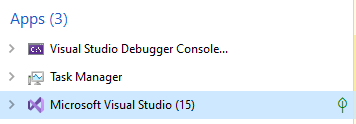
\includegraphics[scale=0.7]{before}
		\caption{Стан до створення процесів}
	\end{figure}
	
	\begin{figure}[H]
		\centering
		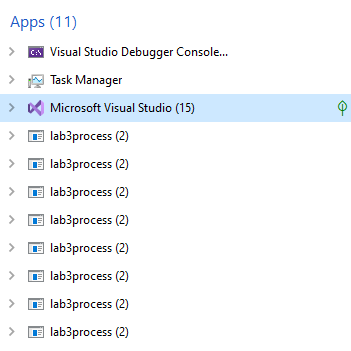
\includegraphics[scale=0.7]{after}
		\caption{Стан після створення процесів}
	\end{figure}
	
	\section*{Висновок}
	Під час виконання лабораторної роботи я ознайомився з багатопоточністю в ОС Windows. Навчився працювати з процесами, використовуючи WinAPI-функції. 
	
	Навчився створювати нові процеси, призупиняти, завершувати та продовжувати їх роботу.
	Навчився отримувати та встановлювати пріоритет процесу за допомогою Win-API функцій.
	Навчився отримувати час виконання процесу за допомогою Win-API функцій.
	
	 
\end{normalsize}
\end{document}
